\section{Related Work and State of the Art}
% \addcontentsline{toc}{section}{Related Work and State of the Art}
\fancyhead[R]{Related Work and State of the Art}

\subsection{Role of Enzymes in Environmental Pesticide Degradation}
\label{sec:Role of Enzymes in Environmental Pesticide Degradation}

The prediction of pesticide degradation and the identification of enzymatic functions involved is a critical area of research with significant implications for environmental sustainability and agricultural practices. As the use of pesticides continues to be a global necessity for crop protection, understanding the mechanisms by which these chemicals are broken down in the environment is essential.

The degradation of pesticides in the environment is a complex process that occurs through various mechanisms, predominantly by microbial enzymatic activities. Enzymes catalyze reactions that transform toxic pesticide compounds into less harmful substances. The most common enzymatic mechanisms involved in pesticide degradation include hydrolytic and oxidative reactions.

For example, reductive enzymes catalyze the reduction of pesticides, in most cases by donating electrons and hydrogen atoms on the molecules. Such a reduction may well break complex structures that facilitate the conversion of pesticides into simpler forms that are much less toxic. For instance, reductive dehalogenases are believed to be important in breaking down halogenated organic compounds.

The application of microbial enzymes in bioremediation strategies has significantly improved the degradation of pesticides in contaminated soils. This approach leverages the natural capability of microbes to detoxify pollutants through enzymatic reactions. Studies have established the efficiency of microbial enzymes in degrading soil-contaminated pesticides. For instance, Singh and Walker \autocite{singhMicrobialDegradationOrganophosphorus2006} highlighted the effectiveness of microbial degradation of organophosphorus compound, while Chia et al. \autocite{chiaFunctionMicrobialEnzymes2024} discussed advancements and applications of microbial enzymes in enhancing biodegradation processes.

Understanding these enzymatic mechanisms is crucial for predicting the enzyme classes responsible for pesticide degradation. By analyzing enzyme-pesticide interactions, it is possible to identify specific enzyme classes involved in the degradation processes. This knowledge can inform the development of more accurate predictive models for pesticide degradation, facilitating better risk assessments and environmental management strategies. Advanced computational methods, such as Deep Learning, can further enhance these predictive models by accurately identifying and classifying enzymes based on their interaction with pesticides, leading to more efficient and targeted development of new products.

\subsection{Deep Learning Techniques in Environmental Science}
\label{sec:Deep Learning Techniques in Environmental Science}

Deep Learning has been an essential tool in environmental science, enabling advanced prediction and understanding complex biochemical processes. There are several Deep Learning architectures such as the protein-transformer ESM model, which has made a significant impact on predicting biological properties from sequence data. \autocite{rivesBiologicalStructureFunction2021}

In the context of pesticide degradation and enzyme classification, such models can analyze large quantities of available biochemical data to make predictions about enzyme interactions and functions. Several deep learning architectures have been applied in enzyme classification and prediction tasks, from which valuable insights into the mechanism of pesticide degradation can be obtained.

For instance, the DEEPre model applies deep learning to predict EC numbers based on raw sequence data. Such models apply convolutional and sequential feature extraction techniques, leading to significant improvements in prediction accuracy over methods in current use. In this respect, such models may play a key role in predicting the pesticide biodegradation pathways and help to make environmental risk assessment more precise and fast. \autocite{liDEEPreSequencebasedEnzyme2017}

The DeEPn model is one of the examples when EC classification has been done using a deep neural network for enzymes being classified into their functional classes, including all seven EC classes. This model has shown high precision and accuracy and, hence could become an essential tool for environmental scientists interested in understanding and predicting enzyme-mediated degradation processes. The proper classification of enzymes through DeEPn can help predict potential candidates for bioremediation, among other applications related to the environment. \autocite{DeEPnDeepNeural}

Despite the advances made by these models, there is still a need for new approaches to further improve the accuracy of sequence based predictions. Traditional models often rely on pre-defined features and limited datasets, which can restrict their performance and generalizability. In addition to this, the existing methods only focus on the prediction to the 3rd level of the EC classification, which may not provide sufficient detail for predicting pesticide degradations.

\begin{figure}[hbt]
    \centering
    \begin{minipage}[t]{.8\textwidth}
    \caption{Macro F1 score for different models and EnzymeNet}
    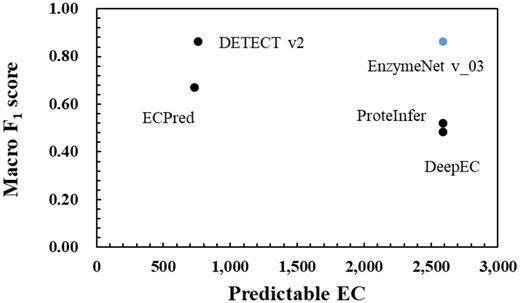
\includegraphics[width=1\textwidth]{img/performance_existing_methods.png}
    \source{Watanabe et al. (2023)}
    \label{fig:EnzymeNet}
    \end{minipage}
\end{figure}

For example the accuracy of EnzymeNet, a residual neural network model, across all the sub-subclasses is 0.398. In addition to that there is no score for the 4th level. The following picture shows the macro F1 score for diffrent models and EnzymeNet, which is the best one, but still not good enough. Therefore, there is a need for more advanced deep learning models that can predict enzyme classes with higher accuracy and resolution, enabling more precise predictions of pesticide degradation pathways. \autocite{watanabeEnzymeNetResidualNeural2023}

By contrast, the proposed approach leverages the deep learning tool p2rank to analyze the interactive parts of enzymes, focusing on the ligand-binding sites and the specific amino acids involved. This method can potentially provide a more detailed and accurate prediction of enzyme classes responsible for pesticide degradation, enhancing our understanding of the biodegradation pathways and mechanisms involved. Furthermore, the emphasis on ligand-binding pockets allows for a more nuanced analysis compared to traditional methods that utilize the entire protein sequence. By concentrating on these critical interaction sites, which are crucial for protein functions, P2Rank can identify the specific residues that are directly involved in the catalytic processes. This specificity could not only improves the accuracy of predictions but also reduce the computational complexity by focusing on smaller, more relevant regions of the protein. \autocite{krivakP2RankMachineLearning2018}